%% SANER 2027 -- Agentic AI4SE Track.
%% Submission: 10 pages + up to 2 pages of references only.
%% Format required by the track: \documentclass[10pt,conference]{IEEEtran}
%% (no compsoc / compsocconf options).
%%
%% ---------------------------------------------------------------------------
%% DOUBLE-ANONYMOUS -- ON. The track desk-rejects submissions that identify
%% their authors, so:
%%   - the author block is "Anonymous Author(s)"; no affiliations, no e-mail
%%   - no repository URL appears anywhere; the artifact is described, not linked
%%   - the earlier version of this work is referred to in the third person and
%%     never cited, so the bibliography carries no self-identifying entry
%%   - no acknowledgments, no funding statement
%% To de-anonymise for the camera-ready, replace the author block and restore
%% the acknowledgments; nothing else in this file needs changing.
%% ---------------------------------------------------------------------------
\documentclass[10pt,conference]{IEEEtran}

\usepackage[T1]{fontenc}
\usepackage{cite}
\usepackage{amsmath}
\usepackage{graphicx}
\usepackage{booktabs}
\usepackage{url}
\usepackage{tikz}
\usepackage[hidelinks]{hyperref}

\emergencystretch=3em
\interdisplaylinepenalty=2500

\begin{document}

\title{When the Benchmark Answers Itself:\\
Two Evaluation Defects in an Agentic RAG Pipeline\\
for Software Ecosystem Update Monitoring}

\author{\IEEEauthorblockN{Anonymous Author(s)}
\IEEEauthorblockA{Affiliations omitted for double-anonymous review}}

\maketitle

\begin{abstract}
A common agentic design decomposes a retrieval-augmented generation (RAG)
pipeline into specialized agents, with a query-rewriting agent normalizing user
terminology to the vocabulary of technical documents. We built such a pipeline for
software ecosystem update questions --- agents for query rewriting, retrieval,
evaluation, and orchestration, with a retrieval-level feedback loop and a
persistent term-weight memory --- and measured a 17.2\% improvement over a
single-agent baseline on a keyword-overlap score of our own design. This paper
reports two evaluation defects that each made that design look decisively better
or worse than the baseline, and what the comparison looks like once both are
removed. Re-scored with standard IR metrics over pooled relevance judgments, the
same system \emph{lost} to the same baseline (nDCG@3 0.145 versus 0.765, $n=10$);
we traced the deficit to a wiring fault, the rewritten query \emph{replacing} the
user's wording at every retrieval endpoint, and repaired it by unioning the pools
of both phrasings. Then a 500-question run scored 0.33 lower than a 300-question
run on the same questions with nothing changed. The benchmark's questions are the
titles of real community posts, the live corpus returns the post a title came
from, and the judge marks it relevant: the question's own source post sat in
72--98\% of the top-$k$ lists behind every number we had reported, and it was
exactly the document a paraphrase loses. Excluded at fetch time, every arm ---
multi-agent, single-agent, and rewrite-only --- retrieves at nDCG@3 0.30--0.31 on
500 questions across 24 ecosystems, with no paired difference above 0.015. A
ranking prior that excluded the community half of the corpus costs every arm a
further 0.227, free to fix and belonging to the retriever rather than to the
agents; with it removed, the two architectures are statistically equivalent on
1{,}000 questions (0.485 versus 0.476) while retrieving almost disjointly, at 50\%
more fetch cost. Each defect was found by a person, and in each case the
automated check that should have caught it was structurally unable to: a unit test
cannot see a fault in the handoff between two correct components, and a paired
test cannot see a bias that inflates every arm equally.
\end{abstract}

\begin{IEEEkeywords}
multi-agent systems, retrieval-augmented generation, query rewriting, retrieval
evaluation, benchmark contamination, software ecosystem monitoring, negative
results, human--agent collaboration
\end{IEEEkeywords}

\section{Introduction}

Modern software ecosystems produce release notes, security advisories, version
control records, and community discussion, and the information a maintainer
needs about an update is usually spread across several of them. Each artefact
has been studied in its own right: release notes are produced inconsistently and
omit what their readers need, which has motivated work on summarising and
generating them~\cite{abebe2016releasenotes,moreno2017arena,bi2022releasenotes},
on characterising their content~\cite{wu2023releasenotes}, and on the discipline
of version identifiers themselves~\cite{guo2025verlog}; the update side is
studied as which strategy a dependent adopts~\cite{javanjafari2023strategies}
and how breaking changes are detected~\cite{kong2025breaking}; and developers
routinely turn to community platforms when documentation is
insufficient~\cite{xia2017websearch,zhang2018apimisuse}, where the reliability
of what they find is an active question~\cite{kabir2024stackoverflow,stolee2025codesearch}.
The task studied here sits across these sources rather than within any one.

Retrieval-augmented generation (RAG) combines document retrieval with a language
model to ground answers in external text~\cite{lewis2020rag}, and is a natural
fit. Single-agent RAG performs query understanding, retrieval, evaluation, and
generation in one reasoning process, which exposes it to vocabulary mismatch
between question and document~\cite{gao2024dmqr}, weak handling of
domain-specific terminology, and the absence of any mechanism for correcting a
retrieval error~\cite{cook2025rag}. Agentic RAG systems therefore decompose
retrieval and reasoning across specialized agents~\cite{wang2024mainrag,nguyen2025marag},
a pattern the broader literature on multi-agent systems for software engineering
surveys in depth~\cite{he2025,liu2026agentsurvey}. We built one for software
update questions: specialized agents for query rewriting, retrieval, evaluation,
and orchestration, connected through a retrieval-level feedback loop and a
persistent term-weight memory.

\subsection{A Result We Did Not Expect}

Our first evaluation followed what is, judging by the literature, common
practice. We defined a retrieval-quality score for the domain --- keyword and
source overlap between the question and the retrieved set --- and compared the
architecture against a single-agent baseline on 50 real user questions. It
improved that score by 17.2\% ($t(49)=2.32$, $p=0.020$), in every question
category. That is the result an earlier version of this work
reported.\footnote{An earlier, peer-reviewed version of this work is referred to
throughout in the third person; the citation is withheld for double-anonymous
review and will be restored in the camera-ready.}

Re-scoring the same pipeline with standard IR metrics --- nDCG@$k$, Recall@$k$,
and MRR over relevance judgments pooled across systems --- reversed the ordering.
The baseline reached nDCG@3 of 0.765; the multi-agent architecture reached 0.145,
a paired deficit of 0.620 (bootstrap 95\% CI $[0.348,0.865]$, exact Wilcoxon
$p=0.016$, $n=10$). A 17.2\% advantage on one metric coexisted with a
factor-of-five deficit on another, over the same questions, the same corpus, and
the same retrieved documents.

Metric disagreements of this size usually mean one metric is measuring something
other than what it claims. That was true here twice over, and neither time in the
direction we assumed. The first investigation produced the diagnosis the first
version of this paper was built around: \emph{the query-rewriting agent's output
replaced the user's wording at every retrieval endpoint, so of the 23 relevant
documents the baseline retrieved, 22 were never fetched by the multi-agent
pipeline at all.} The rewrite was not mis-ordering a correct candidate set --- a
ranking problem, which is how the vocabulary-mismatch framing invites one to read
it --- but constructing a different, smaller candidate set from which the answer
was largely absent. The remedy that implied, issuing both phrasings and unioning
the pools, brought the pipeline to parity at $n=10$, $100$, and $300$.

It was also measuring the wrong thing. The 23 ``relevant documents'' were,
overwhelmingly, the questions' own source posts. The benchmark's questions are the
titles of real community posts, chosen for that reason: they are the questions
people actually asked. The system retrieves from the same live feed those posts
were drawn from. So the feed returns the post a title came from, the judge ---
correctly, by its instructions --- marks a document that \emph{is} the question as
relevant to it, and every retrieval metric rewards the arm that found it. The
baseline, issuing the title verbatim, found it on 7 of the 10 diagnostic
questions; the multi-agent pipeline, issuing a paraphrase, on none. That is the
five-fold deficit.

We found this only because a 500-question run scored 0.33 lower than a
300-question run on the same questions with nothing changed: the leak inflated
every arm equally, so it never appeared in a paired comparison, and surfaced as a
drop in the absolute level when the live feed aged past the source posts
(Section~\ref{sec:leak}). Leak-free, every arm --- including a rewrite-only arm
with no union fetch at all --- retrieves at nDCG@3 0.30--0.31 on 500 questions,
and no paired difference exceeds 0.015.

That substitution harms retrieval is not a new
result~\cite{wang2023query2doc,gao2024dmqr,zighelnic2008drift}, and our
contribution is neither that finding nor its remedy --- nor, after the second
defect, the fetch-loss diagnosis, since the documents the fetch lost turned out to
be the questions. It is the pair of evaluation defects and the order in which they
hid each other: a bespoke metric that rewarded the rewriter's vocabulary made the
architecture look better than the baseline, a benchmark that leaked its own
questions made it look five times worse, and the second defect was invisible to
exactly the paired, pooled-judgment methodology we adopted to escape the first.

\subsection{Research Questions}

The study is organized around five questions, each answered by a measurement in
Section~\ref{sec:results}. \textbf{RQ1:} does decomposing the pipeline into
specialized agents improve retrieval quality over a single-agent baseline on
software update questions (Sections~\ref{sec:leak} and~\ref{sec:tier})?
\textbf{RQ2:} when a domain-specific retrieval score and standard IR metrics
disagree about the ordering of two architectures, what is each measuring, and does
the deficit originate in ranking or in candidate acquisition
(Sections~\ref{sec:two-metrics} and~\ref{sec:localizing})? \textbf{RQ3:} how much
of the reported retrieval quality is attributable to a benchmark whose questions
were mined from the retrieved corpus, and what is the leak-free level
(Section~\ref{sec:leak})? \textbf{RQ4:} which components --- the ranking prior,
the candidate grading cascade, the Orchestrator's retry --- account for measurable
change, which of them belong to the decomposition rather than to the retriever, and
at what cost (Sections~\ref{sec:tier}--\ref{sec:efficiency})? \textbf{RQ5:} which
defects were reachable only by human inspection, and what property of each
automated check made it blind (Section~\ref{sec:human})?

\subsection{Relation to the Earlier Version}

The earlier version contributed the architecture, the bespoke retrieval score,
and the 17.2\% result, which this paper retracts as a metric artifact. New here
are the re-scoring under pooled-judgment IR metrics, the fetch-level diagnosis and
its union-fetch remedy, the discovery and measurement of the benchmark--corpus
leak together with a fetch-time exclusion, leak-free measurements at $n=500$ and
$n=1{,}000$, the ranking-prior and grading-cascade findings, the first measurement
of the Orchestrator's retry, the per-question cost accounting, and the analysis of
where human judgment was structurally required.

\subsection{Contributions}

We contribute: (i) a benchmark--corpus leak specific to live-source RAG, with its
mechanism, a post-hoc correction, a fetch-time exclusion that removes it by
construction, and leak-free measurement at $n=500$ --- in every table we had
previously reported, the question's own post occupied 72--98\% of top-$k$ lists and
was the only judged-relevant document for a third to a half of the questions;
(ii) a reading of query-rewriting drift that the leak reverses, leak-free bringing
a rewrite-only arm within 0.006 nDCG@3 of a verbatim baseline, together with
evidence that a bespoke retrieval metric can invert the architectural conclusion
and that pooled-judgment IR metrics over a leaking corpus measure a lookup rate;
(iii) an honest accounting of what decomposition bought --- equivalence within
$\pm0.02$ nDCG@3 at $n=500$ and $n=1{,}000$, at twice the latency and up to 16
times the model calls --- alongside a ranking prior worth $+0.227$ to \emph{both}
arms at no additional model call, and the first measurement of the Orchestrator's
retry, whose gate its own quality signal cannot open; and (iv) an account of where
human judgment was required, derived from the defects rather than asserted: four
blind spots, each a sound automated check that was structurally unable to see
outside its own frame.

\section{Related Work}\label{sec:related}

\textbf{Retrieval-augmented generation.} RAG grounds generation in retrieved
documents~\cite{lewis2020rag}. Extensions address limitations of a fixed
pipeline: DMQR-RAG rewrites queries to reduce vocabulary
mismatch~\cite{gao2024dmqr}, RaFe adds feedback-based
reranking~\cite{ma2023rafe}, Self-RAG adds self-evaluation during
generation~\cite{asai2024selfrag}, and Adaptive-RAG selects retrieval logic per
query~\cite{jeong2024adaptiverag}; surveys identify adaptive retrieval and
agent-based coordination as active directions~\cite{gao2023survey}.

\textbf{Query rewriting and expansion.} The standard justification is vocabulary
mismatch~\cite{furnas1987vocabulary}, addressed classically by expanding the query
from an initial retrieved set~\cite{rocchio1971relevance} or from corpus-wide
co-occurrence~\cite{xu1996localglobal,carpineto2012survey}. Language models made
the expansion text cheap to generate: HyDE retrieves with the embedding of a
hypothetical answer document~\cite{gao2023hyde}, query2doc concatenates a
pseudo-document with the original query and reports that the generated text alone
underperforms no rewriting at all~\cite{wang2023query2doc}, and prompting
strategies for expansion have been compared against pseudo-relevance
feedback~\cite{jagerman2023expansion}. Zighelnic and Kurland establish both the
drift risk and the fusion remedy~\cite{zighelnic2008drift}. Our fetch-level
finding re-observes theirs inside an agentic pipeline; what is new is what the lost
documents turned out to be.

\textbf{Agentic RAG and multi-agent SE.} MAIN-RAG and related systems decompose
retrieval and filtering across agents~\cite{wang2024mainrag,nguyen2025marag},
MetaGPT formalises role decomposition~\cite{hong2024metagpt}, benchmarks such as
SWE-bench measure end-task success~\cite{jimenez2024swebench}, and GPTSwarm
studies agent graphs as optimisable structures~\cite{zhuge2024}; recent surveys
catalogue agentic SE systems and their evaluation
gaps~\cite{he2025,liu2026agentsurvey,mamun2026blagent,guan2025,zheng2026,yang2026}.
HULA places the human at fixed handoff points rather than at points the agent
selects by self-assessment~\cite{takerngsaksiri2025hula}; our retry result
(Section~\ref{sec:retry}) is an argument for that choice.

\textbf{Evaluation methodology.} BEIR established zero-shot retrieval evaluation
across heterogeneous corpora~\cite{thakur2021beir} and dense retrievers are now
standard baselines~\cite{izacard2022contriever}. LLM relevance judges order
systems about as well as human assessors while agreeing poorly per
label~\cite{upadhyay2024umbrela,thomas2024preferences,faggioli2023perspectives},
and can be fooled by query-string injection in ways $\kappa$ does not
predict~\cite{alaofi2024fooled}; Section~\ref{sec:threats} bounds our threats with
these figures rather than against them.

\textbf{Benchmark leakage.} The leak we report is a relative of the contamination
problem in language-model evaluation, where benchmark items appear in a model's
pre-training data and inflate measured
performance~\cite{sainz2023contamination}, and of code duplication in machine
learning for software engineering, where near-identical files across the
train/test split inflate reported accuracy~\cite{allamanis2019duplication}. Two
properties distinguish it. It is not in the model's weights but in the
\emph{retrieval corpus at inference time}, so no decontamination of training data
removes it and no held-out split protects against it; and it inflates every arm
equally, so the paired, pooled-judgment protocol that the IR literature
recommends --- and that we adopted --- is precisely the protocol that cannot see
it. We are not aware of a prior report of this failure mode for live-source RAG,
and we give the mechanism, its magnitude in our own published numbers, and a
fetch-time exclusion in Section~\ref{sec:leak}.

\section{Architecture}\label{sec:method}

The architecture separates software update question answering into four agents
under a central Orchestrator (Fig.~\ref{fig:architecture}), following five
principles: one task per agent; retrieval restricted to vendor-specific sources
when a vendor can be identified; retrieval quality assessed by an explicit
mechanism that can trigger another attempt; failures isolated by input/output
contracts; and retrieval outcomes persisted across sessions so adaptation needs
no human feedback.

\begin{figure}[t]
\centering
\resizebox{0.95\columnwidth}{!}{%
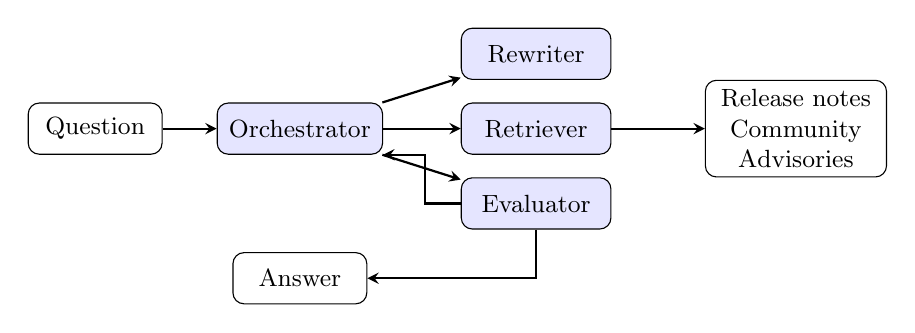
\begin{tikzpicture}[
  box/.style={rectangle,draw,rounded corners,text centered,align=center,
              minimum height=0.65cm,font=\small,fill=white},
  agent/.style={box,fill=blue!10},
  arrow/.style={->,thick,>=stealth}]
\node[box,minimum width=1.7cm] (user) at (0,0) {Question};
\node[agent,minimum width=2.1cm] (orch) at (2.6,0) {Orchestrator};
\node[agent,minimum width=1.9cm] (rw) at (5.6,0.95) {Rewriter};
\node[agent,minimum width=1.9cm] (ret) at (5.6,0) {Retriever};
\node[agent,minimum width=1.9cm] (eval) at (5.6,-0.95) {Evaluator};
\node[box,minimum width=2.3cm] (docs) at (8.9,0)
  {Release notes\\ Community\\ Advisories};
\node[box,minimum width=1.7cm] (ans) at (2.6,-1.9) {Answer};
\draw[arrow] (user) -- (orch);
\draw[arrow] (orch) -- (rw);
\draw[arrow] (orch) -- (ret);
\draw[arrow] (orch) -- (eval);
\draw[arrow] (ret) -- (docs);
\draw[arrow] (eval.south) |- (ans.east);
\draw[arrow] (eval.west) -- ++(-0.45,0) |- (orch.south east);
\end{tikzpicture}}
\caption{The architecture. The Evaluator scores retrieval quality and can return
control to the Orchestrator for a retry before an answer is generated;
Section~\ref{sec:retry} reports that this gate cannot open.}
\label{fig:architecture}
\end{figure}

\textbf{Orchestrator.} Receives the question, delegates to the other agents, and
manages retrieval retries when the Evaluator requests one; it neither retrieves
nor generates. \textbf{Query Rewriter.} Transforms the question into a
retrieval-oriented restatement of at most 20 words directed at bug fixes,
releases, changelogs, security patches, and performance, using Llama~3.1~8B, with
learned terms from previous retrieval outcomes prepended in the self-improving
configuration. \textbf{Retriever.} Identifies the vendor by exact, alias, and
fuzzy matching against a registry of product names and subreddits fetched at
startup, restricts retrieval to that vendor's release notes, advisories, and
community discussions when one is found, and returns ranked documents without
assessing their quality. \textbf{Evaluator.} Scores retrieval quality
deterministically in $[0,1]$ from retrieval volume, release-note matches,
community matches, and CVE matches, and signals a retry below a threshold
($\theta=0.15$ in the released implementation); Section~\ref{sec:retry} reports
that this gate cannot open.

\textbf{Adaptation.} A persistent Self-Improvement Memory accumulates positive and
negative scores for query expansion terms across sessions, which the Rewriter
consults, adapting retrieval without preference labels or retraining. No
measurement reported here exercises it, and the retry loop is inactive in
Sections~\ref{sec:two-metrics}--\ref{sec:leak}; we state this rather than let the
architecture description stand in for the measured system.

\subsection{Two Roles for a Rewritten Query}

A rewritten query serves two purposes whose requirements are in tension. Issued to
an endpoint, its job is to \emph{widen} the candidate set: vendor synonyms, product
aliases, and release-note vocabulary admit documents the user's phrasing would not
reach. Used to \emph{order} that set, its job would be to express what the user
asked --- which by construction it no longer does. One rule follows, applied
throughout the Retriever:

\begin{quote}
\emph{The rewritten query determines what is fetched. The original question
determines how it is ordered.}
\end{quote}

Let $q$ be the user's question and $\tilde{q}$ the rewrite. Candidate
acquisition is parameterized by both; ranking by $q$ alone. Vendor
identification runs on $q$, because rewrites reliably inject the tokens
\texttt{release}, \texttt{update} and \texttt{fixes}, which the vendor registry
matches as product names.

\subsection{Candidate Acquisition by Union Fetch}\label{sec:union-fetch}

Let $\mathcal{E}$ be the retrieval endpoints and $R_e(x)$ the documents endpoint
$e$ returns for a phrasing $x$. The Retriever searches
\begin{equation}
Q = \begin{cases}
\{\tilde{q}\} & \text{if } \mathrm{fold}(q) = \mathrm{fold}(\tilde{q}),\\
\{\tilde{q},\, q\} & \text{otherwise,}
\end{cases}
\label{eq:phrasings}
\end{equation}
where $\mathrm{fold}(\cdot)$ is whitespace-trimmed lower-casing, and the raw
candidate multiset is
\begin{equation}
C = \bigcup_{e \in \mathcal{E}(q,\tilde{q})} \; \bigcup_{x \in Q} R_e(x).
\label{eq:union}
\end{equation}
Equation~\eqref{eq:phrasings} is what leaves the baseline unaffected: the
baseline passes the same string as both phrasings, $Q$ collapses, and
Equation~\eqref{eq:union} reduces to the pre-existing behaviour, so the
comparison is a before/after on the multi-agent arm alone. $C$ is deduplicated
by URL, falling back to $\mathrm{fold}(\mathrm{title} \,\|\, \mathrm{source})$
for feeds that omit one, order-preservingly and per trust tier, with the verified
tier's keys pre-seeded into the community pass so a document reachable from both
appears only in the higher tier. The pool $P$ is recorded per question, so that
``the reranker mis-ordered it'' and ``it was never fetched'' remain separable
diagnoses --- the instrumentation both defects were eventually found with. The
union adds one request per phrasing-parameterized endpoint and none for the vendor
release lookup, which is keyed on the vendor name: requests rise from 13 to 24
for a question with a recognised vendor, and from 7 to 14 without one. No
additional model calls are incurred, since the Rewriter runs once either way.

\subsection{Ranking}\label{sec:rerank}

Ranking is a separate, replaceable stage scored against $q$. A reranker sees the
concatenation of title, body, top-voted community comment, and subreddit --- the
same text the synthesizer is shown, so ranking and synthesis cannot disagree
about what a document says. Each tier is sorted by descending score, the sorted
tiers are concatenated, and the cut to top-$k$ ($k=4$) is applied once at the
end. Three backends are selected by environment variable, so the choice is an
ablation arm rather than an assumption: \texttt{none}, a substring boost on the
head tokens of the ranking query, which reproduces the published configuration;
\texttt{bm25}, Okapi BM25 with $k_1=1.5$, $b=0.75$, computed over the pool being
ordered rather than a global corpus, with a tokenizer that keeps version strings
whole so that \texttt{v6.18.21} and \texttt{6.18.21} match; and \texttt{embed},
cosine similarity under \texttt{nomic-embed-text} served locally through Ollama. A
backend that cannot reach its model degrades to BM25 but flags the run, so a
results table cannot attribute a lexical run to a semantic backend.
Section~\ref{sec:tier} reports that sorting \emph{within} tier --- the decision
in this paragraph --- costs more than every architectural difference in this
paper combined.

\section{Evaluation Protocol}\label{sec:setup}

\textbf{Question sets.} Three sets answer different questions. The
\emph{original} set is 50 update questions spanning security, bug, release,
community, and general maintenance topics, on which the superseded bespoke score
was measured. The \emph{ground-truth} set is 10 questions carrying reference
answers, used for the diagnostic measurements of
Sections~\ref{sec:two-metrics}--\ref{sec:localizing} because document-level
counting is tractable at that size. The \emph{benchmark} is mined from real
community threads across 24 software ecosystems, stratified by category and
ecosystem, in nested sets of 100, 300, 500 and 1{,}000, each a strict prefix of
the next; 445 of the 500 questions are the titles of real posts, and each
carries the URL of the post it came from --- the record that makes the leak of
Section~\ref{sec:leak} both possible and detectable. Sample sizes are stated
with every number.

\textbf{Baseline.} The single-agent baseline issues the question directly and
performs retrieval, evaluation, and generation in one agent, with no rewriting,
retry, or memory. It uses the same endpoints and the same synthesis prompt as
the proposed architecture, isolating architectural decomposition.

\textbf{Arms.} Two arms are comparable only when one capability separates them,
so the ablation is a ladder in which each rung adds exactly one capability:
\texttt{raw} (no retrieval); \texttt{single\_agent} (retrieval on the user's
question); \texttt{single\_agent\_grounded} (question grounding, no coordination);
\texttt{rewrite\_only} (rewriting, no union); \texttt{marag\_llm} (union fetch
over both phrasings); \texttt{marag\_llm\_retry} (Orchestrator retry); and
\texttt{marag} (the Evaluator's template rendering). The \texttt{marag\_llm} arm
exists so that answer-quality scores are comparable: it is \texttt{marag}'s
retrieval synthesized through the baseline's own prompt.

\textbf{Measures.} Relevance is judged on a graded 0--2 scale (not relevant /
partially relevant / highly relevant), from which nDCG@$k$, Recall@$k$, and MRR
are computed over the pooled judgments at $k \in \{1,3,5\}$ with a top-$k$ cut of
$k=4$ in the pipeline. Answer quality uses two RAGAS-style judged
scores~\cite{es2024ragas}: \emph{faithfulness}, the share of an answer's claims
supported by its retrieved documents, and \emph{answer relevance}, how well the
answer addresses the question. On the subset of questions carrying a reference
answer, \emph{correctness} is scored in the CRAG style~\cite{yang2024}, which
treats an abstention differently from a wrong answer, so an arm that declines on a
question yields no scoreable prediction rather than a zero. The superseded bespoke
score is the Evaluator's own keyword- and source-overlap measure
(Section~\ref{sec:method}), reported only where the comparison with it is the
point. Latency is wall-clock per question, reported as a median.

\textbf{Judging and models.} Relevance labels are graded and \emph{pooled}: every
document any arm retrieved for a question is judged once and the label reused for
every arm that retrieved it, so no arm is scored against a private set of
judgments. Unless stated otherwise, generation and judging use Llama~3.1~8B
through Ollama at temperature zero on Apple Silicon with 24\,GB of memory; the
ladder synthesizes with Mistral and judges with \texttt{qwen2.5:7b-instruct}, and
the grading cascade of Section~\ref{sec:tier} grades candidates with
\texttt{qwen2.5:7b-instruct}. Where a measurement is described as frozen, every
arm was served from a corpus snapshot recorded in a preceding pass and replayed,
so all arms saw byte-identical documents.

\section{Results}\label{sec:results}

\subsection{Two Metrics, Two Orderings}\label{sec:two-metrics}

The bespoke score is a keyword- and source-overlap measure between the question
and the retrieved set, computed by the Evaluator. Under it the multi-agent
architecture improved on the baseline in all five question categories, from
0.680 to 0.798 --- a 17.2\% relative improvement, paired $t(49)=2.32$, $p=0.020$.
Re-scored with pooled-judgment IR metrics on the ten ground-truth questions, the
ordering reverses, and not marginally: the baseline reaches nDCG@1 0.800, nDCG@3
0.765 and MRR 0.800, the multi-agent arm 0.133, 0.145 and 0.250, for paired
differences of $-0.667$, $-0.620$ and $-0.550$ at exact two-sided Wilcoxon $p$ of
0.016, 0.016 and 0.031.

Because the bespoke score rewards overlap between question and retrieved set
without reference to whether a retrieved document answers the question, it can
be maximized by retrieving many topically adjacent documents. The multi-agent
arm is worse on seven of the ten questions and tied on three, never better; the
mean paired nDCG@3 difference is $-0.620$ (percentile bootstrap 95\% CI
$[-0.865,-0.348]$~\cite{efron1993bootstrap}, exact Wilcoxon
$p=0.016$~\cite{wilcoxon1945}, $d_z=-1.39$~\cite{cohen1988power}), and every
metric agrees in direction at $p \le 0.031$.

Two caveats bound this, and we state them because $n=10$ makes both
load-bearing. The Wilcoxon test discards ties, leaving seven pairs, for which the
smallest attainable two-sided $p$ is $2/2^{7}=0.0156$; the observed $p$ \emph{is}
that floor, so the correct reading is that every non-tied question favours the
baseline, not that the evidence would survive a stricter threshold. And the
intervals place the deficit between roughly a third and nine tenths of the
metric's range: they establish sign and order of magnitude, not magnitude. A third
caveat, learned later and larger than both, is that the IR columns measure how
often an arm retrieved the question's own source post --- 7 of 10 for the
baseline, 0 of 10 for the multi-agent arm. Leak-free the same run reads 0.397
against 0.263: the ordering survives, the factor of five does not.

\subsection{Localizing the Loss}\label{sec:localizing}

A deficit of this size has two candidate explanations --- appropriate documents
ordered badly, or documents not retrieved --- and they call for different fixes.
A ranking ablation separates them. With only
the rewritten phrasing retrieved, three successively stronger ranking functions
raise MRR monotonically from 0.250 to 0.625 while nDCG@3 stays near 0.19: the
ranker is correctly ordering a candidate set that does not contain the answer.
With both phrasings retrieved and the pools merged, every configuration improves
sharply, and the choice of which phrasing to \emph{rank} against is worth 0.024
nDCG@3 against the four-fold effect of which to \emph{retrieve} with. An
intervention that improves the metric it targets while leaving the outcome
metric unchanged is addressing a real but secondary defect --- a diagnostic we
think generalizes.

We therefore stopped inferring from scores and counted documents. Of the 23
relevant documents the baseline retrieved, \textbf{22 were never retrieved by
the multi-agent pipeline at all}. The cause is a wiring property, not a
modelling one: every endpoint was issued the rewritten query \emph{instead of}
the user's question, and the rewrite is a lossy paraphrase by design. No
reranker can promote a document that was never fetched.

On the repaired pipeline, over 100 benchmark questions against a frozen corpus,
the same progression of ranking functions raises nDCG@3 by 0.170 and MRR by
0.198 together --- the signature is absent once the fetch is repaired, which is
how a diagnosis of this form is falsifiable. Two further readings come from that
run: mean candidate-pool recall is 0.981 for the multi-agent arm against 0.839
for the baseline, so the union does raise the ceiling reranking can reach; and
the choice of ranking function (0.170) matters more than the choice of
architecture (never above 0.021).

\subsection{The Own-Post Leak}\label{sec:leak}

Everything above was measured on a corpus that contained the questions.

\textbf{How it surfaced.} Extending the 300-question run to 500 by the same
procedure, from the same cache and seed, the baseline's nDCG@3 on the 300 shared
questions fell from 0.818 to 0.494 and the multi-agent arm's from 0.827 to
0.483. Nothing in the pipeline had changed. A uniform drop of 0.33 on every arm,
on identical questions, is not a systems effect.

\textbf{Mechanism.} The harness derives a document's identifier from its URL, so
the post the feed returns is the same document the benchmark record points to,
and the judge --- asked whether a document is relevant to a question --- marks
the document that \emph{is} the question as relevant. In the 300-question run
the own post was in the pool for 247 of the 262 community-mined questions,
judged relevant for 232, and the \emph{only} judged-relevant document for 140.
Two weeks later the feed had aged past most of them: 171 of 445 in the pool, the
only relevant document for 82. The score fell with the leak.

The property that made it hard to see is that every arm issuing the user's
phrasing retrieves the own post at the same rate --- 72--73\% of top-$k$ lists on
the frozen 100-question corpus, 82--83\% on the live 300, 98\% on the frozen
scaled replay --- so the paired differences, which is what every statistical test
in this paper computes, never contained it. It appears only in the absolute level,
and only across runs, which the frozen-corpus protocol we adopted for
comparability specifically discourages. The one arm that does not issue the user's
phrasing is \texttt{rewrite\_only}, which retrieves the own post 4\% of the time;
that is the whole of the 0.21-against-0.73 contrast we had read as rewriting
collapsing retrieval.

\textbf{Correction.} Table~\ref{tab:leak} strikes the own post from every arm's
ranked list and from the judgments and recomputes each retrieval measurement in
this paper. Two things in it are the point. The leak-free column is nearly flat:
a system whose reported retrieval quality ranged from 0.15 to 0.92 depending on
the table has, on documents that are not the question, retrieved at roughly 0.3
throughout. And the corrections preserve every parity result while reversing the
drift result: the arms stay within 0.015 of each other in every sample, and
\texttt{rewrite\_only}, 0.52 behind the baseline as reported, is 0.006 behind it
leak-free, with 8 questions better and 9 worse.

\begin{table}[t]
\caption{Every retrieval measurement in this paper, as reported and with the
question's own source post struck from ranking and judgments. ``Own post'' is the
share of that arm's ranked lists containing it.}
\label{tab:leak}
\centering
\footnotesize
\setlength{\tabcolsep}{3.5pt}
\begin{tabular}{@{}llrrr@{}}
\toprule
Sample & Arm & nDCG@3 & leak-free & own post \\
\midrule
$n{=}10$ diagnostic & single & 0.736 & 0.397 & 7/10 \\
                & multi  & 0.145 & 0.263 & 0/10 \\
$n{=}10$ rewrite only & multi & 0.188 & 0.309 & 0/10 \\
$n{=}10$ union fetch & multi & 0.765 & 0.216 & 10/10 \\
$n{=}100$ frozen & single & 0.924 & 0.331 & 98\% \\
                 & multi  & 0.922 & 0.320 & 98\% \\
$n{=}100$ ladder & single & 0.731 & 0.269 & 72\% \\
                 & grounded & 0.780 & 0.321 & 73\% \\
                 & rewrite-only & 0.210 & 0.263 & 4\% \\
                 & multi & 0.752 & 0.267 & 73\% \\
$n{=}300$ live & single & 0.818 & 0.324 & 82\% \\
               & multi  & 0.827 & 0.319 & 83\% \\
$n{=}500$ live & single & 0.494 & 0.309 & 34\% \\
               & multi  & 0.483 & 0.294 & 34\% \\
\bottomrule
\end{tabular}
\end{table}

\textbf{Fetch-time exclusion.} Post-hoc correction changes the score but not
what the systems saw: an arm that retrieved the own post spent a top-$k$ slot on
it, and the judge's other labels were pooled from lists containing it. We
therefore struck the question's own URL from every arm's candidate pool before
ranking, recorded that the run did so, and re-ran the 500 questions with nothing
else changed. The own post appeared in none of the 445 pools.
Table~\ref{tab:clean} is the result, and three readings follow.

\begin{table}[t]
\caption{The 500-question benchmark with the own post excluded at fetch time.
Lower rows give the paired difference against the single-agent baseline,
win/tie/loss over questions, and the Holm-corrected $p$~\cite{holm1979}. Latency is
a per-question median.}
\label{tab:clean}
\centering
\footnotesize
\setlength{\tabcolsep}{3pt}
\begin{tabular}{@{}lrrrrr@{}}
\toprule
System & nDCG@3 & Rec@5 & MRR & Faith. & Lat. \\
\midrule
\texttt{marag} (templ.) & 0.304 & 0.351 & 0.344 & 0.844 & 53.9 \\
\texttt{marag\_llm} (prose) & 0.306 & 0.353 & 0.345 & 0.915 & 53.6 \\
\texttt{single\_agent} & 0.301 & 0.366 & 0.344 & 0.910 & 26.4 \\
\midrule
$\Delta$ \texttt{marag} & $+0.003$ & $-0.015$ & $0.000$ & $\mathbf{-0.066}$ & \\
\quad W/T/L & 40/418/42 & 39/408/53 & 28/434/38 & 28/189/283 & \\
\quad $p_{\mathrm{Holm}}$ & 1.000 & 0.654 & 1.000 & $\mathbf{<}\mathbf{0.001}$ & \\
$\Delta$ \texttt{marag\_llm} & $+0.004$ & $-0.013$ & $+0.001$ & $+0.005$ & \\
\quad W/T/L & 39/419/42 & 39/409/52 & 28/434/38 & 79/364/57 & \\
\quad $p_{\mathrm{Holm}}$ & 1.000 & 0.654 & 1.000 & 0.376 & \\
\bottomrule
\end{tabular}
\end{table}

\emph{The honest retrieval figure is about 0.30, for every arm.} On 273 of the 500
questions no arm's pool contains a document the judge marks relevant: for most
questions people actually ask about software updates, the live release, advisory,
and community feeds do not contain an answer, and no arm changes that. Parity
should be read against that ceiling.

\emph{Parity is exact, and it is not the arms retrieving the same documents.} Only
113 of 500 top-$k$ lists are identical across the two architectures, and the
multi-agent pool averages 19.3 documents against the baseline's 12.8: the pipeline
fetches half again as many candidates, different ones, and no retrieval metric
moves by more than 0.015. This is the one result that survived every correction in
this paper unchanged, at $n=10$, 100, 300, and 500, leaking and leak-free.

\emph{The format effect is real and smaller than the leaking runs made it.}
Template rendering costs 0.066 faithfulness here (283 worse, 28 better,
$p<0.001$) against 0.110 in the leaking 500-question run and 0.196 at $n=300$;
part of the earlier gap was the template rendering the own post's title verbatim
under a ``verified'' banner. The same retrieval rendered as prose is
indistinguishable from the baseline ($+0.005$, $p=0.38$). On a frozen
100-question ladder the cost is $0.095$ under multi-agent retrieval and $0.102$
under single-agent retrieval, both $p<0.0001$ --- the same magnitude in both
cells, which confirms it as a property of the rendering and not of the
architecture. Any comparison that places a template arm against a prose arm
measures this before it measures retrieval.

One number in the clean run we decline to report as a result. On the 72 questions
with a reference answer the template arm scores 0.129 higher on correctness than
either prose arm ($p=0.002$). Reading the winning answers, they \emph{decline} ---
they state that the sources do not cover the question, the same abstention the
prose arms make --- under a ``VERIFIED from live APIs'' header and a list of
version strings, and the judge scores that 0.7 against a reference the answer does
not contain. The measurement is sound and it is measuring presentation.

\subsection{A Ranking Prior That Excluded the Corpus}\label{sec:tier}

Parity at a low absolute number admits two readings: the arms are equally good,
or equally obstructed by something neither controls. The second was right.

\textbf{Mechanism.} The Retriever ranks \emph{within} source tiers before the
top-$k$ cut, so every verified record precedes every community post whatever the
scorer says. The comment justifying the ordering referred to the ``verified
sources'' block of the answer template --- a rendering concern --- but the
ordering was applied to retrieval. The consequence is arithmetic: across the 500
questions the top-4 of every arm is 0\% community posts, on a question set that
is 60\% community-mined. The multi-agent pool held 455 judged-relevant documents
to the baseline's 425 and left 48 of them outside its top-4, against the
baseline's 6; ranked by an oracle the same two pools score 0.419 and 0.389. The
retrieval advantage the union produces exists in the pool, and the prior
discards it before the metric can see it.

\textbf{Offline re-ranking.} We re-ranked the recorded pools of the clean run with every
scoring function the system implements, in both modes, judging the 3{,}142
additional documents any new ranker promoted into a top-4 the incumbent had never
shown the judge, so that a ranker is not scored zero for surfacing something no
previous configuration exposed. Every tiered configuration sits between 0.15 and
0.25 (\texttt{bm25} 0.153, \texttt{rrf} 0.221, \texttt{llm} 0.238,
\texttt{embed} 0.250 as run) and every flat one between 0.32 and 0.49
(\texttt{bm25} 0.322, \texttt{rrf} 0.410, \texttt{embed} 0.458,
\texttt{llm20@embed} 0.489): the choice of scoring function --- lexical, dense,
fused, or model-graded --- moves the metric less than the single decision of
whether to apply the prior at all. The baseline's pools move the same way
(\texttt{tiered:embed} 0.248 to \texttt{flat:embed} 0.452), and strict relevance,
grade 2 only, tells the same story lower, 0.087 to 0.176. Three successive
reranker generations in Section~\ref{sec:localizing} were evaluated against a
ceiling that was not the reranker's to reach.

\textbf{End to end.} On 100 questions stratified by category against one frozen
snapshot with nothing changed but the prior, \texttt{marag\_llm} goes from 0.357
to 0.584 and \texttt{single\_agent} from 0.388 to 0.616: both arms gain an
identical $+0.227$ (95\% CI $[+0.146,+0.316]$ and $[+0.144,+0.319]$), which is
what makes this a defect fix rather than an architectural result. Fixing it
benefits a single agent exactly as much as four. Two costs come with it:
faithfulness falls 0.022 and 0.026 and answer relevance 0.026 and 0.034, because
the flat top-4 is 38\% community posts and 17\% news, and a model answering from
community text answers from weaker ground than one answering from a vendor
advisory. The obvious follow-up is not available: removing news costs 0.14 nDCG@3,
because 58\% of news documents are judged relevant and 24\% highly relevant. News
is the most relevant source in this corpus.

\textbf{One lever is the agents'.} Reading the candidate documents --- grading the
top 20 with a local model and re-sorting the head by grade, the Evaluator's natural
job --- improves ranking where counting sources did not: $+0.027$ nDCG@3 over
\texttt{flat:embed} (95\% CI $[+0.016,+0.039]$, 57 wins to 20 losses, $n=500$) at
20 model calls per question. It is the mechanism by which a larger pool could in
principle be cashed: under the enlarged judgments the multi-agent union holds
1{,}439 judged-relevant documents to the baseline's 1{,}232, 303 of them fetched by
the multi-agent arm alone.

Run end to end on all 500 questions with flat ranking and the cascade on the
multi-agent arm, that arm appeared to lead on every rank-sensitive metric: nDCG@1
$+0.049$, nDCG@3 $+0.032$, MRR $+0.025$, each with an interval excluding zero and
surviving Holm correction. We report those numbers because they are wrong, and the
error is one an evaluation of this kind invites. The two arms did not run in the
same pass: the multi-agent arm came from a run that queried the endpoints live and
recorded them, the baseline from a strict replay of that recording. A snapshot
holds one response per request key and a live feed answers the same key
differently over the hours a 500-question run takes --- replaying the
live-recorded run reproduced its pools on 1 of 12 questions where two replays of
one configuration agree on 12 of 12 --- so the comparison graded an arm that had
seen a wider, fresher community feed against one that had not. A control that
gives the baseline the same cascade does not improve it (nDCG@3 $0.479 \to 0.467$,
interval spanning zero; recall@5 $-0.035$ with one that does not), so reading
candidates is not worth 20 model calls to an arm with nothing extra in its pool to
promote; against that control the multi-agent arm led by $+0.044$, inheriting the
confound. Table~\ref{tab:control} removes it, and is null.

\begin{table}[t]
\caption{All three arms in one pass: 500 questions, flat ranking, grading cascade
on every arm, strict replay of one snapshot. Paired, percentile bootstrap 95\% CI,
Holm-corrected.}
\label{tab:control}
\centering
\footnotesize
\setlength{\tabcolsep}{3pt}
\begin{tabular}{@{}lrrll@{}}
\toprule
Metric & Multi & Single & $\Delta$ (95\% CI) & W/T/L \\
\midrule
nDCG@1 & 0.462 & 0.445 & $+0.017\,[-0.001,+0.035]$ & 17/475/8 \\
nDCG@3 & 0.496 & 0.490 & $+0.006\,[-0.009,+0.021]$ & 43/410/47 \\
nDCG@5 & 0.509 & 0.499 & $+0.010\,[-0.004,+0.025]$ & 56/390/54 \\
Recall@5 & 0.551 & 0.532 & $+0.018\,[-0.001,+0.038]$ & 46/426/28 \\
MRR & 0.536 & 0.528 & $+0.008\,[-0.004,+0.022]$ & 22/457/21 \\
\midrule
Faithfulness & 0.900 & 0.897 & $+0.003\,[-0.006,+0.012]$ & 72/375/53 \\
Ans.\ rel. & 0.950 & 0.948 & $+0.002\,[-0.007,+0.011]$ & 55/408/37 \\
\bottomrule
\end{tabular}
\end{table}

With the prior removed, the cascade on both arms, one corpus, one judge, one
clock, and one pass, the multi-agent architecture does not beat the baseline on
any retrieval metric. The largest difference is $+0.018$ recall@5, whose interval
includes zero and which does not survive correction; nDCG@3 is $+0.006$ with 43
won and 47 lost. Both halves of the earlier story survive on their own terms ---
the prior cost every arm 0.23, and grading candidates improves ranking --- and
what does not survive is the claim that the multi-agent arm converts them into an
advantage. Nothing has changed from Section~\ref{sec:leak} except the absolute
level: every arm now retrieves at roughly 0.49 rather than 0.30.

Measured again at twice the scale, on the full 1{,}000-question benchmark with
flat ranking and an embedding reranker on all three arms in one pass, the answer
is the same: nDCG@3 0.485 for both multi-agent arms against 0.476 for the
baseline, paired $+0.009$ $[-0.003,+0.021]$, win/tie/loss 101/796/103. Doubling
the sample moves the absolute level not at all and the gap not at all, which is
what a null looks like when it is not a power problem. The two arms are not doing
the same work beneath that score: their candidate pools are identical on 1
question of the 1{,}000, the multi-agent pool is half again as large (18.6
documents against 12.4), and the top-4 the ranker returns is identical on 264. The
tie is two systems retrieving differently --- one at 50\% more fetch cost --- and
arriving at the same place. A strict replay returned the same retrieved set and
the same full candidate pool for all 3{,}000 arm--question pairs against 51{,}245
document reads, with every retrieval metric matching to four decimals.

\textbf{Equivalence rather than an underpowered null.} A null result invites the
objection that the study lacked power to detect a real effect, so we state the
bound the intervals give. At $n=500$ the 95\% CI on the paired nDCG@3 difference is
$[-0.009,+0.021]$ and at $n=1{,}000$ it is $[-0.003,+0.021]$: effects larger than
about $0.02$ nDCG@3 --- 4\% relative to the level both arms reach --- are excluded
in both directions, and the bound does not shrink when the sample doubles, which is
what distinguishes equivalence from insufficient data. The largest architectural
difference anywhere in this paper, $+0.018$ Recall@5, is smaller than the
$+0.055$ Recall@5 gap we obtained from nothing but a difference in which arms the
judgments were pooled across (Section~\ref{sec:retry}), and smaller by an order of
magnitude than the $+0.227$ the ranking prior is worth. We therefore read the
comparison as equivalence within roughly $\pm 0.02$ nDCG@3, not as a question the
data leaves open.

The rule we would offer is narrow and mechanical, because the confounded
comparison was not careless --- each run was internally frozen, the judgments
pooled, the statistics paired and corrected --- and it still produced a significant
result with a plausible mechanism. What it lacked was one pass: in a live-corpus
domain, two arms compared against each other must execute in the same run, and the
only way to be sure is to make the run frozen and reproducible and then reproduce
it.

\subsection{The Retry That Could Not Fire}\label{sec:retry}

Parity leaves one capability unmeasured, and it is the one a single agent
structurally lacks: the Orchestrator's adaptive retry. Across 500 frozen
questions the Evaluator's quality score has a minimum of exactly 0.300 and the
retry fires below 0.15; the arm returned candidate lists identical to
\texttt{marag\_llm} on 500 of 500 questions and answers identical on 500 of 500.
Zero retries fired.

The exact minimum is the tell. The Evaluator does not compute a quality score so
much as raise one through a ladder of floors: a verified advisory source sets it
to at least 0.30, community posts to 0.50, release notes to 0.50, both together
to 0.65. Any retrieval returning one recognised document is floored at twice the
threshold, and the union fetch returns one for every question in this benchmark.
The gate is not conservative; it is closed. A retry can occur only when
retrieval comes back empty, which is the one case a wider re-fetch is least
likely to repair. Reporting this rung as a measured null would have been the
more flattering error: it would suggest adaptive retrieval was tested and found
neutral, when what was tested was a threshold the scoring function makes
unreachable.

The released implementation reads the retry signal from the term-overlap score
\emph{before} the floors are applied, leaving the reported score and the
threshold untouched. Under that reading the retry fires on 94 of 500 questions
and changes the top-4 on 71 of them --- and every metric is flat: nDCG@3
$-0.002$ $[-0.013,+0.008]$, recall@5 $-0.001$, faithfulness $+0.002$, with
win/loss splits as close to even as the counts allow. The Orchestrator's second
round is neither inert nor cosmetic: it asks the Rewriter for vocabulary the
first round did not try, fetches on it, and brings back different documents for
one question in five. Those documents are on average neither better nor worse
than the ones they displaced. Adaptive retrieval as this system implements it
re-rolls the dice rather than improving the odds, and a re-roll is what a null of
this shape looks like: motion without direction.

One comparison came free. The retry arm judged only its own candidates while
\texttt{marag\_llm} was judged inside a three-arm pool, and the two retrieved
byte-identical lists on every question: scored as each run reports itself they
differ by $+0.055$ Recall@5, and re-scored against the union of both runs'
judgments by $0.000$. That gap, from nothing but the company the judgments kept, is
larger than every architectural difference this paper reports.

\subsection{What the Accuracy Costs}\label{sec:efficiency}

A retrieval improvement reported without its price is not a result a
practitioner can act on. The harness counts every generation and token each arm
spends on its own work, excluding the judge, with each configuration measured
alone in its own process over the same 25 questions against the same snapshot
. ``Cold'' below is the first question of a
process; the mean over 25 is lower because the grading cascade caches a grade per
(question, document) pair, a property of the corpus rather than of the
architecture, so a deployed system answering unrelated questions pays the cold
price. Single-agent, \texttt{flat:embed}: 1 generation and 315 tokens per question
(cold 1 / 332). Single-agent, \texttt{flat:llm20@embed}: 12.6 and 2{,}984 (cold 22
/ 5{,}033), nDCG@3 0.490. Multi-agent, \texttt{flat:embed}: 3.0 and 1{,}105 (cold
3 / 1{,}199). Multi-agent, \texttt{flat:llm20@embed}: 16.4 and 4{,}192 (cold 23 /
6{,}012), nDCG@3 0.496.

Decomposition without the cascade costs 3 generations to the baseline's 1: the
Rewriter, answer synthesis, and one we report rather than defend --- the Evaluator
assembles its template unconditionally and the template embeds an answer the prose
arm then discards, so roughly 900 tokens per question are paid for and thrown away
in every multi-agent measurement here. The cascade costs about 12 generations and
2{,}700 tokens per question and buys neither architecture a lead over the other.
The best configuration costs 16 times the calls and 13 times the tokens of the
cheapest and retrieves indistinguishably from the baseline. The practitioner's
conclusion rather than the architectural one: if retrieval quality at minimum cost
is the objective, the single-agent baseline with flat ranking and an embedding
reranker is the configuration to deploy, and the one intervention in this paper
that is both large and free is the removal of the tier prior --- $+0.227$ nDCG@3
for every arm, at no additional model call at all.

\section{Extension: A Decision Layer for Update Triage}\label{sec:decision-layer}

A later, less formally evaluated extension of the pipeline, \texttt{decide()},
moves from what a maintainer should \emph{read} to what they should \emph{do}:
an agentic verdict over live vendor feeds, community discussion, and the CISA
KEV catalogue, in place of a static CVE lookup. We report it briefly, not as a
result on par with Section~\ref{sec:results}, because its central failure is a
further instance of what Section~\ref{sec:human} describes: a component that
was individually correct produced a confidently wrong answer at a handoff that
no automated check could catch.

\textbf{A false-green safety verdict.}\label{sec:false-green}
The decision layer answered \emph{safe} to ``is it safe to update Firefox right
now,'' badged green, while 11 Firefox advisories were live, one eight days old.
Two independent gates each had to fail for this; fixing either alone left the
bug in place. First, the intent classifier reads ``is it safe/good/stable''
as an \emph{opinion} question, and the citation rule for opinion questions
excludes advisories --- so the verdict, computed over that same citable set,
never saw them and fell through to \emph{safe} with rationale ``no advisory.''
The fix carries advisory rows to the verdict regardless of intent, leaving the
citation rule in force only for what the prose may describe. Second, even with
advisories reaching the verdict, the live NVD feed phrases most records
\emph{weakness-first} --- naming the product only in a ``\ldots fixed in
Firefox 157.0.1'' clause, never the sentence's subject --- so the rule matching
an advisory to the asked-about product rejected these as off-topic and
reconstructed the same green verdict from otherwise-correct data. The fix
accepts a product named in that fix clause under the same cross-vendor guard
already in place, which also keeps a macOS question from crediting macOS with
an advisory for a third-party tool merely running on it (we also fixed an
unrelated \texttt{isCve}/\texttt{is\_cve} key mismatch that had silently
misclassified advisories as releases).

\texttt{patch\_urgently} is unchanged at 22/200 on the frozen benchmark before
and after the second fix --- it adds live-feed coverage without moving an
already-scored verdict --- while the live Firefox query now returns
\texttt{patch\_urgently} instead of \texttt{insufficient\_evidence}. Separately,
61 of the 200 questions are phrased as release or opinion questions that
structurally exclude CVE records, leaving \texttt{patch\_urgently} unreachable
for 30.5\% of the sheet regardless of evidence, independent of this bug.

\textbf{Parametric memory versus a live advisory feed.}\label{sec:update-order-baseline}
How much of the update urgency a live feed measures is already encoded in a
general-purpose LLM's training-time knowledge? We ranked the 30 ecosystem
components tracked throughout this work twice: once by the pipeline's live
severity-weighted advisory count (\texttt{monitor.risk}, ReleaseTrain/NVD) and
once by a local Llama~3.1~8B, through Ollama, with no retrieval, ordering the
same 30 by urgency from its own knowledge. The full ranking is in the
supplementary material (Table~S13).

Agreement is statistically indistinguishable from zero: Spearman's
$\rho=-0.050$, Kendall's $\tau=-0.039$; treating $\rho$ as a test statistic,
$t(28)=-0.26$, $p\approx0.79$. The two rankings disagree most sharply at the
extremes, in opposite directions. The live feed places \texttt{linux} at rank 2
--- 126 advisories in the trailing 90 days, second only to \texttt{wordpress}'s
299 --- while the model ranks it last, 30th; the reverse holds for the database
cluster, where the model ranks \texttt{postgresql}, \texttt{mysql}, and
\texttt{mongodb} 1st--3rd as a category prior while the live feed shows almost
no current advisory activity against them (\texttt{mongodb} at rank 29). The
one region of agreement, the browser cluster, does not move the global
correlation, since the kernel and database inversions pull opposite ways and
largely cancel.

We read this as a static training-time prior with no mechanism to notice that
this quarter's advisory stream disagrees with it, not as the two systems
weighting the same evidence differently. At $n=30$ this $\rho$ is not reliably
distinguishable from a random pairing, so the reading is not a precise
anti-correlation estimate; it is that substituting parametric memory for a
live feed in a security-adjacent decision would, here, rank the single
highest-advisory-volume component as the lowest priority. One baseline model,
one run --- hosted models and repeated sampling are the natural next step.

\section{Discussion}\label{sec:discussion}

\subsection{What Generalizes}

Two findings compete for the one most likely to transfer; the second qualifies the
first.

The first: \emph{a rewriting agent must add to the retrieval it performs, not
substitute for it.} The distinction is easy to lose because it is invisible in the
agent's own output. A rewritten query inspected in isolation looks correct --- it
names the vendor, uses release-note vocabulary, reads like a well-formed search ---
and what is invisible at that level is that issuing it \emph{instead of} the user's
question silently and unrecoverably narrows the candidate set, which
Section~\ref{sec:human} reads as a property of agentic pipelines rather than of
this one. The general diagnostic is worth stating on its own: when an intervention
improves the metric it targets while leaving the outcome metric unchanged, it is
addressing a real but secondary defect.

The second: \emph{a benchmark mined from the sources a system retrieves from
contains its own answer key.} The property that makes live-source RAG attractive
for software ecosystems --- the corpus is the current state of the feeds, not a
snapshot --- is the property that lets a question mined from those feeds retrieve
itself, and we expect this in any evaluation whose questions and corpus are drawn
from the same live population: forums, issue trackers, mailing lists, changelogs.
Three properties of it transfer. It is \emph{invisible to paired comparison},
since pooled judging, frozen corpora, and Holm-corrected tests all worked exactly
as intended on a quantity that was mostly a lookup. It is \emph{selectively
visible to arms that do not issue the user's wording}, so any intervention that
changes the query string --- rewriting, expansion, translation,
decontextualization --- will show a spurious deficit against a verbatim baseline,
with the textbook signature of query drift. And its \emph{detection signal is an
absolute level that moves when it should not}: had we reported absolute levels
alongside paired deltas and re-run identical questions at an interval, the leak was
visible at $n=10$. Leak-free, substituting the rewrite for the question costs 0.006
nDCG@3 --- which is what the second finding does to the magnitude of the first.

\subsection{Where the Human Was Required}\label{sec:human}

This paper reports four defects. Each was found by a person, and in each case the
automation that should have found it was not merely absent but \emph{structurally
incapable}. We are not reporting a study of human--AI collaboration: no
participants were recruited and no interaction was measured. What follows is a
retrospective account of a system that was built, measured, corrected, and
measured again, read for what the automation could not do for itself.

\textbf{Component testing cannot see a wiring fault.} The defect lived in what
one agent handed another, and 22 of 23 relevant documents were never fetched. No
unit test of any component fails on this, because no component is wrong. One
question makes the seam visible on its own: asked ``What was the Linux version on
January 1st 2026?'', the pipeline carried the date constraint correctly through
the rewriter and dropped it at the retrieval call --- the rewriter preserved it,
the retriever was never given it, and neither violated its contract. What a user
sees is an answer about the wrong release; what a per-component test sees is two
components passing. The fault is visible only from a position holding both sides
of the handoff at once, and no agent in the pipeline occupies that position.

\textbf{The system's own quality signal can move the wrong way with
confidence.} The bespoke score rose 17.2\% when the architecture was introduced
--- the number a designer checks --- while measuring the correlation between a
metric and the vocabulary the rewriting agent produced. An agent cannot audit a
measure whose blind spot it occupies.

\textbf{Paired statistics cannot see a bias that inflates every arm equally.} The
leak appeared only in the absolute level, the one thing a frozen-corpus protocol
teaches practitioners not to compare across runs, and it was caught because a
person noticed that the same 300 questions scored 0.33 lower two weeks later and
treated a moving level as a finding rather than as noise. \textbf{And a coherent
explanation absorbs the evidence against it}: the literature, the mechanism, and
the measurement agreed, and nothing in the pipeline was positioned to distrust a
story that fit.

\textbf{The agent cannot ask for help it cannot recognise needing.} The
escalation mechanism is the capability a single agent structurally lacks, and its
gate is closed by construction (Section~\ref{sec:retry}). The general form is
worth separating from our implementation: a self-assessment built from the same
evidence the system already trusts will tend to be confident exactly where the
system is wrong, because the failure and the confidence have a common cause, and
an escalation path conditioned on that self-assessment inherits the blindness.
This is the mechanism behind the familiar complaint that agentic systems fail
silently rather than asking, expressed here as a measurement: a threshold the
scoring function makes unreachable, and a rung of an ablation ladder that could
not execute as built. Frameworks that place the person at fixed handoff points
rather than at points the agent selects~\cite{takerngsaksiri2025hula} are, on
this evidence, right to do so for retrieval as well.

\textbf{Two capabilities no metric here scores} exist for a person rather than
for a benchmark. \emph{Traceability}: when an answer is wrong, the decomposition
localises the fault to vendor extraction, reformulation, retrieval coverage,
evaluation, or synthesis, and for a system meant to be maintained rather than
benchmarked once, answering ``which stage failed'' is what makes the next repair
possible. \emph{Abstention}: on most questions no arm retrieves a document the judge accepts
(Section~\ref{sec:leak}), and returning ``the retrieved sources do not answer
this'' is a hand-back that tells a person the question needs them --- preferable,
in a maintenance context, to a confident wrong version number.

\textbf{Evaluation is the loop that did not close.} All judgments here were
produced by \texttt{llama3.1}, which also synthesises two of the three arms.
Re-scoring every judgment with a different model family leaves the ordering intact
and every paired difference's sign unchanged, at per-label Cohen's
$\kappa=0.370$~\cite{cohen1960coefficient}: the ordering survived automated
replacement, the labels did not agree, and two language models cannot settle that
between themselves. What the limit costs is concrete, and this paper contains the
case --- the template arm's 0.129 correctness advantage is sound, reproducible,
architecturally flattering, and measuring a header. No aggregate could have caught
it, because the aggregate is what was fooled, and no second automated judge
settles it, because the format that misleads one model is available to mislead
another. Someone had to open the answers and read them.

Each automated check was sound within its own frame --- the unit test about its
component, the metric about its retrieved set, the paired test about its
difference, the literature about its mechanism --- and each was blind outside it.
The human contributions were not better versions of those checks but changes of
frame: inspect the seam rather than the part, count documents rather than read
scores, treat a moving absolute level as evidence, and hold a fitting explanation
open. Instrumenting for the frame change is therefore as important as instrumenting
for the task: expose the pre-ranking candidate set so that ``mis-ordered'' and
``never retrieved'' are separable without reading code; report absolute levels
alongside paired deltas; and treat a self-assessment that never triggers as a defect
report rather than as evidence of health.

\section{Threats to Validity}\label{sec:threats}

\textbf{Construct validity.} Both measures of retrieval quality in this paper ---
the bespoke score and pooled-judgment IR metrics --- turned out to measure
something other than retrieval of answers
(Sections~\ref{sec:two-metrics}, \ref{sec:leak}). The leak-free figures exclude the
question's own source post but not near-duplicates of it --- cross-posts,
quotations, or aggregator copies under a different URL --- so the 0.30 level is an
upper bound on retrieval of independent evidence.

\textbf{LLM relevance judge.} All judgments were produced by \texttt{llama3.1},
which is also the synthesis model --- the circularity condition the IR literature
warns about --- and we did not measure agreement with human assessors on our
corpus. Published figures suggest such labels are usable for \emph{ordering}
systems and weak per item: run-level Kendall's $\tau$ of 0.77 to
0.94~\cite{upadhyay2024umbrela,thomas2024preferences} against per-label $\kappa$
near 0.26 to 0.37~\cite{upadhyay2024umbrela,faggioli2023perspectives}, so the
claims we draw are ordering claims and document counts, not calibrated
effectiveness estimates. LLM judges over-label
relevance~\cite{alaofi2024fooled}, which inflates the denominator of the 22-of-23
census, though its direction is unaffected because those documents were absent
from the multi-agent pool regardless of their label; and LLM qrels carry less
discriminative power than human ones~\cite{faggioli2023perspectives}, so the
significance in Section~\ref{sec:two-metrics} was obtained under a handicap rather
than assisted by one. We re-judged the answer-quality finding with \texttt{qwen2.5:7b-instruct} on 40
questions (the format effect holds at $+0.107$ versus $+0.111$) and re-scored all
2{,}446 retrieval pairs behind Table~\ref{tab:control} with \texttt{mistral}, a
different family with no part in that run: every paired difference keeps its sign,
three of four shrink, and agreement is $\kappa=0.370$ graded, $0.421$ binary. The
disagreement runs one way --- \texttt{mistral} judges 14.5\% of the pool relevant
against \texttt{llama3.1}'s 33.2\% --- so the judges disagree about where the
threshold sits, not about which documents are better, which is why absolute levels
halve while every ordering holds. The equivalence result is robust to the choice of
judge; it is not evidence that a stronger one would agree, since no human-assessor
sample was drawn.

\textbf{Benchmark validity.} The questions are real, and that is the source of the
leak: they were mined from the population the system retrieves from. A benchmark
constructed to avoid it --- questions from a source the corpus cannot return, or a
corpus frozen before the questions were posted --- would measure a different,
harder task, and we have not built one. On the present benchmark 273 of 500
questions have no judged-relevant document in any arm's pool, so more than half of
it measures abstention behaviour rather than retrieval.

\textbf{Internal and external validity.} The baseline shares the proposed system's
endpoints and synthesis prompt, isolating decomposition; implementation details
such as alias coverage, endpoint freshness, and rewriting quality may still
influence the comparison. The equivalence result rests on 1{,}000 questions, the
leak-free measurement on 500, the diagnostics on 10 --- all English-language, over
24 ecosystems and public sources, and small against real workloads. Results may
differ for other languages and ecosystems, enterprise repositories, or domains
where release documentation and community discussion are thin.

\section{Conclusion}

We presented a multi-agent RAG architecture for software update questions and an
account of what happened when we measured it properly. On a keyword-overlap score
of our own design it improved on a single-agent baseline by 17.2\%; under standard
IR metrics over pooled judgments it lost to the same baseline by roughly a factor
of five. We traced that deficit to the rewriting agent's output being issued to
every endpoint \emph{in place of} the user's question and repaired it by unioning
the pools --- and then found that the documents the repair recovered were the
questions themselves, returned by a live corpus the benchmark had been mined from.

Leak-free, every arm retrieves at nDCG@3 0.30 on 500 questions across 24
ecosystems; with a ranking prior removed that cost every arm a further 0.227, every
arm retrieves at 0.49; and at $n=500$ and $n=1{,}000$ the two architectures are
equivalent within $\pm0.02$ nDCG@3 while their candidate pools barely intersect, at
50\% more fetch cost. Decomposition did not improve retrieval quality over a
well-configured single-agent baseline here, and neither did the repair we had built
for it. We suggest that agentic pipelines expose the pre-ranking candidate set,
that evaluations on live corpora report absolute levels alongside paired deltas and
re-run identical questions at an interval, and that a benchmark mined from a
system's own sources be assumed to leak until the question's source document is
shown absent from every pool. Those instruments lower a cost; they do not remove a
person. Every defect here was found by one, and in each case the check that should
have caught it was structurally unable to see outside its own frame. Future work
includes head-to-head comparison against Self-RAG, CRAG, and Adaptive-RAG; a
human-assessor sample and a stronger independent judge; and larger, multilingual
question sets over longer interaction
histories~\cite{yang2024,ranaldi2025,reuter2025}. The architecture, the harness
with the own-post exclusion built in, the ablation arms, the script that recomputes
any earlier run leak-free, and the 500-question benchmark are available to
reviewers as an anonymized artifact on request, and will be published on
acceptance.

\section*{Generative AI Disclosure}

Llama~3.1, Mistral, \texttt{nomic-embed-text} and \texttt{qwen2.5:7b-instruct},
run locally through Ollama, are components of the system under study and perform
rewriting, synthesis, judging, embedding and candidate grading as reported; those
uses are measurements. Separately, an AI coding assistant helped implement the
harness, analyse run artifacts, and draft and revise portions of this manuscript.
Every design decision, retraction and interpretation is the authors', who verified
each reported number against the artifacts that produced it. No AI system is listed
as an author.

\bibliographystyle{IEEEtran}
\bibliography{references}

\end{document}
